\documentclass[a4paper,10pt,landscape,twocolumn]{scrartcl}

%% Settings
\newcommand\problemset{6}
\newcommand\worksession{Tuesday, 17 October 2017}
\newif\ifcomments
\commentsfalse % hide comments
%\commentstrue % show comments

%% Packages
\usepackage[english]{exercises}
\usepackage{wasysym}
\usepackage{hyperref}
\hypersetup{colorlinks=true, urlcolor = blue, linkcolor = blue}
\usepackage{enumitem}
\usepackage{graphicx}

%% Macros
\usepackage{xspace}

\newcommand{\eps}{\varepsilon}
\newcommand{\ket}[1]{|#1\rangle}
\newcommand{\bra}[1]{\langle#1|}
\newcommand{\inp}[2]{\langle{#1}|{#2}\rangle}
\newcommand{\norm}[1]{\parallel\!#1\!\parallel}
\newcommand{\points}[1]{\marginpar{\textbb{#1 p.}}}
\newtheorem{theorem}{Theorem}
\newtheorem{definition}{Definition}
\newtheorem{proposition}{Proposition}
%\newenvironment{proof}{\noindent {\bf Proof }}{{\hfill $\Box$}\\}

\newcommand{\gen}{\ensuremath{\mathsf{Gen}}\xspace}
\newcommand{\enc}{\ensuremath{\mathsf{Enc}}\xspace}
\newcommand{\dec}{\ensuremath{\mathsf{Dec}}\xspace}
\newcommand{\mac}{\ensuremath{\mathsf{Mac}}\xspace}
\newcommand{\vrfy}{\ensuremath{\mathsf{Vrfy}}\xspace}
\newcommand{\negl}{\ensuremath{\mathsf{negl}}\xspace}
\newcommand{\PrivK}{\ensuremath{\mathsf{PrivK}}\xspace}
\newcommand{\eav}{\ensuremath{\mathsf{eav}}\xspace}

\newcommand{\Z}{\ensuremath{\mathbb{Z}}}
\newcommand{\R}{\ensuremath{\mathbb{R}}}
\newcommand{\N}{\ensuremath{\mathbb{N}}}


\newcommand\floor[1]{\lfloor#1\rfloor}
\newcommand\ceil[1]{\lceil#1\rceil}

% \newcommand{\comment}[1]{{\sf [#1]}\marginpar[\hfill !!!]{!!!}}
\newcommand{\chris}[1]{\comment{\color{blue}Chris: #1}}
\newcommand{\jan}[1]{\comment{\color{magenta}Jan: #1}}




\begin{document}

\problems


\begin{exercise}[El Gamal encryption]
As in Example 11.17 in [KL], let $\mathbb{G}$ be the subgroup of $\mathbb{Z}_{167}^*$ generated by $g=4$. We have that the order $q=|\mathbb{G}|=83$ is prime. Let the secret key be $x=23 \in \Z_{83}$ and so the public key is $pk = \langle p,q,g,h \rangle = \langle p,q,g,g^x \rangle$ 
\begin{subex}
Compute the $h$ component in the public key.
\end{subex}
\begin{subex}
Compute the encryption of message $m=19 \in \mathbb{G}$ with randomness $y=44$.
\end{subex}
\begin{subex}
Decrypt the ciphertext $\langle c_1,c_2 \rangle = \langle 132,44 \rangle$.
\end{subex}
\end{exercise}

\begin{exercise}[RSA]
\begin{subex}[RSA encryption]
As in Example 11.27 in [KL], say $\mathsf{GenRSA}$ outputs $(N,e,d)=(1005973,89,d)$. Note that $1005973=997 \cdot 1009$.
\begin{enumerate}
\item Encrypt the message $m=1234 \in \Z_{1005973}^*$
\item Compute the private key $(N,d)$ corresponding to the public key $(N,e)=(1005973,89)$.
\item Decrypt the ciphertext $c=530339$.
\end{enumerate}
\end{subex}


{
  \centering
  \begin{figure}
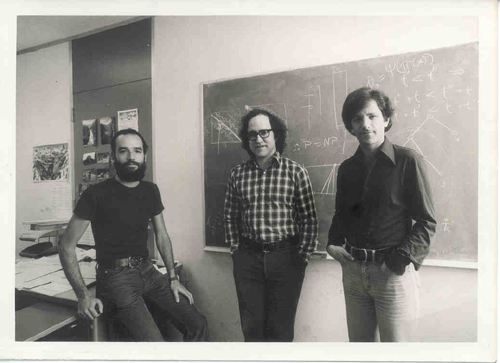
\includegraphics[height=0.15\textwidth]{RSA-MIT.jpg}
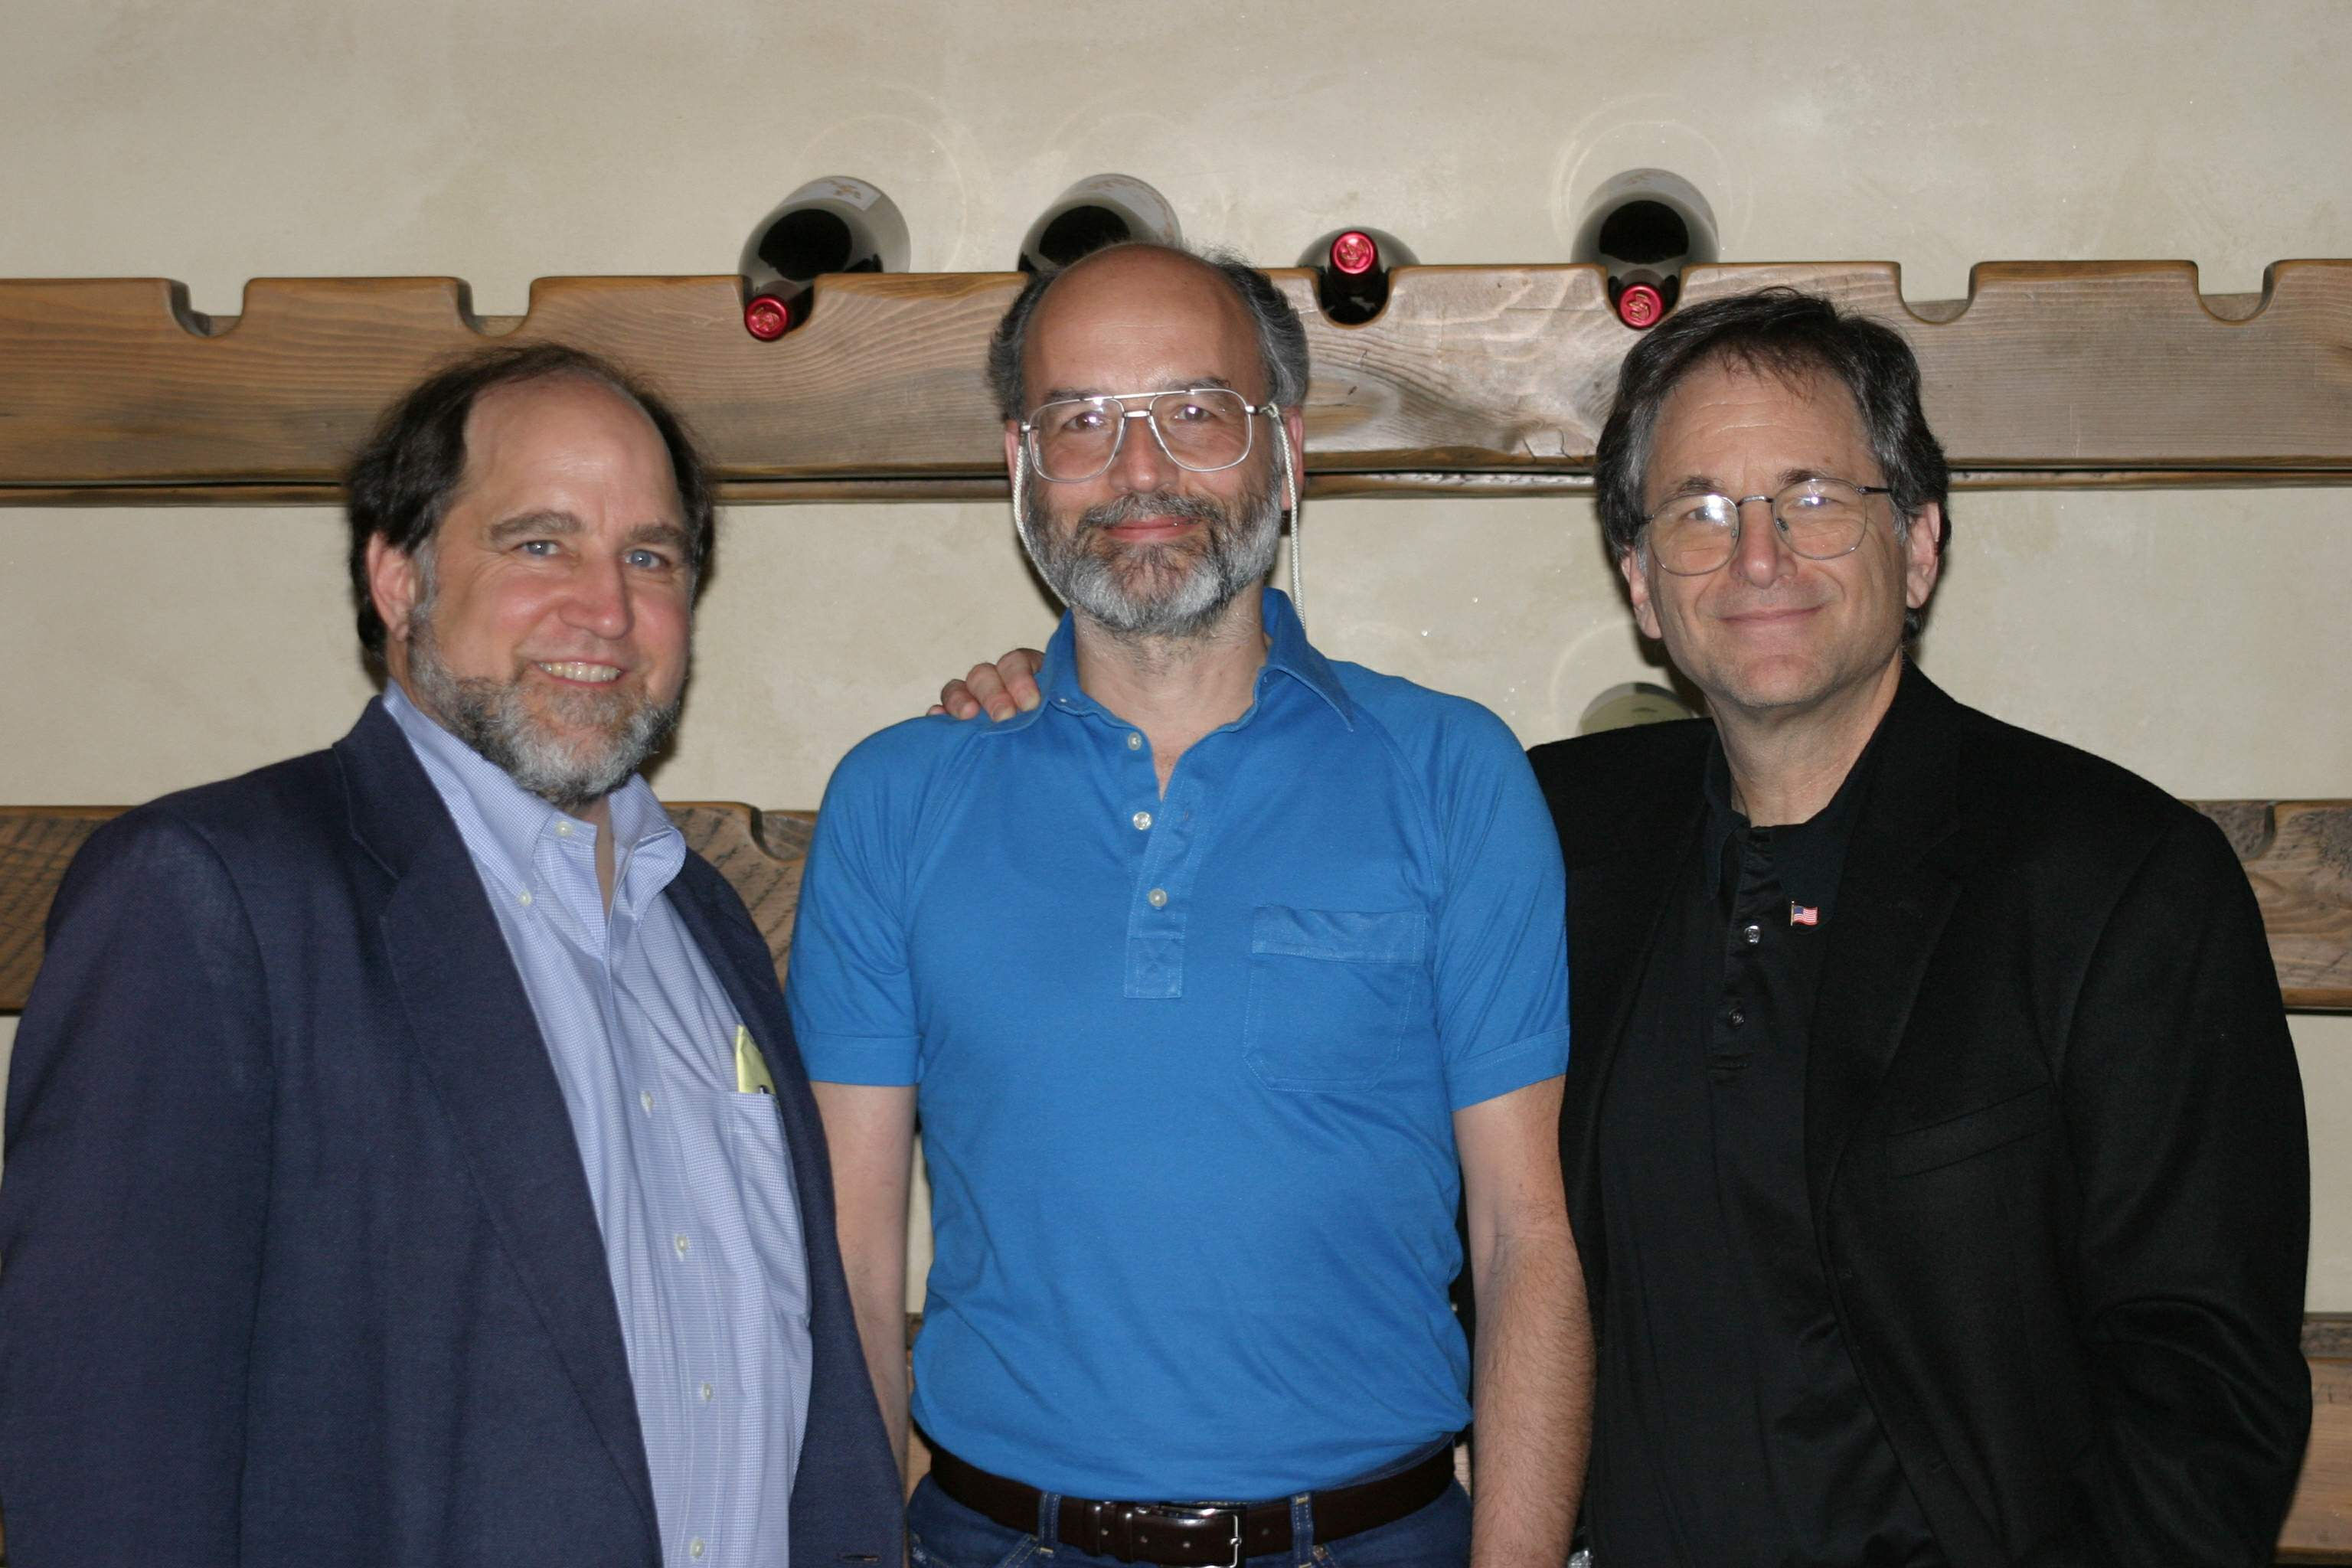
\includegraphics[height=0.15\textwidth]{RSA-2003.jpg}
\caption{Adi Shamir, Ron Rivest, and Len Adleman as MIT-students and in 2003\newline
{\small Image credit:
  \url{http://www.ams.org/samplings/feature-column/fcarc-internet},
  \url{http://www.usc.edu/dept/molecular-science/RSA-2003.htm}}}
\end{figure}
}

\begin{subex}[Attacks on Plain RSA]
\begin{enumerate}
\item For the RSA public key $(N,e)=(10000799791, 3)$, decrypt the ciphertext $c=1 000 000$. Can you do it without factoring $N$?
\item Suppose we would like to use plain RSA with public exponent $e=3$ as public-key encryption in a hybrid scheme together with AES-256 in CBC mode. We choose $N$ to have roughly 2048 bits. Use the previous subexercise to argue the insecurity of this hybrid scheme.
\end{enumerate}
\end{subex}
\end{exercise}



	
%\pagebreak
\begin{exercise}[CCA security of multiple encryptions]
Claim 11.7 in [KL] states that if $\Pi=(\mathsf{Gen},\mathsf{Enc}, \mathsf{Dec})$ is a CPA-secure public-key encryption scheme for fixed-length messages, then the new encryption scheme $\Pi'=(\mathsf{Gen},\mathsf{Enc}', \mathsf{Dec}')$ with  $\mathsf{Enc}'_{pk}(m_1\|m_2\|...\|m_\ell)=\mathsf{Enc}_{pk}(m_1)\|\mathsf{Enc}_{pk}(m_2)\|...\|\mathsf{Enc}_{pk}(m_\ell)$ is CPA secure for arbitrary-length messages.

	Show that Claim 11.7 does not hold in the setting of CCA-security: Exhibit a concrete attack on a scheme $\Pi'=(\mathsf{Gen},\mathsf{Enc}', \mathsf{Dec}')$ constructed from a fixed-length CCA secure encryption scheme $\Pi=(\mathsf{Gen},\mathsf{Enc}, \mathsf{Dec})$ by defining 
\[ \mathsf{Enc}'_{pk}(m_1\|m_2\|...\|m_\ell)=\mathsf{Enc}_{pk}(m_1)\|\mathsf{Enc}_{pk}(m_2)\|...\|\mathsf{Enc}_{pk}(m_\ell) \]
\end{exercise}



\newpage

\begin{exercise}[RSA Signatures]
\begin{subex}[Plain RSA Signatures]
Say the public key is $\langle N,e \rangle=\langle 91,11\rangle$.
\begin{enumerate}
\item Verify that $(43,36)$ is a valid message-signature pair.
\item Compute $\phi(N)$.
\item Calculate the private key $d$.
\item Sign the message $m=28$.
\end{enumerate}
\end{subex}

\begin{subex}[Insecurity of plain RSA Signatures]

In Section 12.4.1 we showed an attack on the
plain RSA signature scheme in which an attacker forges a signature
on an arbitrary message using two signing queries. Show how an
attacker can forge a signature on an arbitrary message using a
\emph{single} signing query.

\textbf{Hint:} Use the no-query and the two-query attacks. 
\end{subex}

% \begin{subex}[Plain RSA Signatures, weaker definition]
% Assume the RSA problem is hard. Show that the plain RSA signature scheme satisfies the following weak definition of security: an attacker is given the public key $\langle N, e\rangle$ and a uniform message $m \in \mathbb{Z}^*_N$. The adversary succeeds if it can output a valid signature on $m$ without making any signing queries.
% \end{subex}
\end{exercise}


\begin{exercise}[One-time-secure signature scheme?]
A signature scheme is one-time-secure if no PPT adversary making a \emph{single} query can output a valid forgery.

Let $f$ be a one-way permutation (it is hard to calculate the inverse of $f$). Consider the following signature
scheme for messages in the set $\{1,\dots , n\}$:
\begin{itemize}
\item To generate keys, choose uniform $x \in \{0, 1\}^n$ and set $y := f^{(n)} (x)$
(where $f^{(i)}(.)$ refers to $i$-fold iteration of $f$, and $f^{(0)} (x) = x$). The
public key is $y$ and the private key is $x$.
\item To sign message $i \in \{1,\dots , n\}$, output $f^{(n-i)} (x)$.
\item To verify signature $\sigma$ on message $i$ with respect to public key $y$,
check whether $y = f^{(i)} (\sigma)$.
\end{itemize}

\begin{subex}
Show that the verification procedure will output 1 for every legal message-signature pair.
\end{subex}
\begin{subex}
Show that the above is not a one-time-secure signature scheme.
Given a signature on a message $i$, for what messages $j$ can an
adversary output a forgery?
\end{subex}
\begin{subex}
Prove that no PPT adversary given a signature on $i$ can output a
forgery on any message $j > i$ except with negligible probability.
\end{subex}
\end{exercise}

\begin{exercise}[El-Gamal variant]
	Consider the following public-key encryption scheme. The public key is $(G,q,g,h)$ and the private key is $x$, generated exactly as in the El-Gamal encryption scheme. In order to encrypt a bit $b$, the sender does the following:
	\begin{enumerate}
		\item If $b=0$ then choose independent random $y,z \leftarrow \mathbb{Z}_q$, compute $c_1 = g^y$ and $c_2 = g^z$, and set the ciphertext equal to $(c_1, c_2)$.
		\item If $b = 1$ then choose a random $y\leftarrow \mathbb{Z}_q$ and compute $c_1 =g^y$ and $c_2 = h^y$. The ciphertext is $(c_1, c_2)$.
	\end{enumerate}
	Show that it is possible to decrypt efficiently given knowledge of $x$. Prove that this encryption scheme is CPA-secure if the decisional Diffie-Hellman problem is hard relative to $\mathcal{G}$.
\end{exercise}


\newpage

\begin{bonusexercise}[Perfectly secure public-key encryption?]
	Assume a public-key encryption scheme for single-bit messages with no
	decryption error. Show that, given $pk$ and a ciphertext $c$ computed via
	$c=\mathsf{Enc}_{pk}(m)$, it is possible for an unbounded adversary to determine
	$m$ with probability 1.
\end{bonusexercise}


\begin{bonusexercise}[Another one-time secure signature scheme]
Let $f$ be a permutation and $f^{(i)}(x)$ the $i$-fold iteration of $f$,
and $f^{(0)}(x) := x$. Let us consider the following signature scheme
$\Pi = (\mathsf{Gen},\mathsf{Sign},\mathsf{Vrfy})$ for messages $m \in \{1, \ldots, p\}$ with $p = p(n)$ polynomial in $n$.
\begin{center}\vspace{-1em}
\begin{tabular}{rcl}
  $\mathsf{Gen}(1^n)$ & : &
    Choose $\mathsf{sk}_1,\mathsf{sk}_2 \in_R \{0,1\}^n$, $\mathsf{pk}_1 := f^p(\mathsf{sk}_1)$ and $\mathsf{pk}_2 := f^p(\mathsf{sk}_2)$. \\
    & & Set $\mathsf{sk} := (\mathsf{sk}_1,\mathsf{sk}_2)$ and $\mathsf{pk} := (\mathsf{pk}_1,\mathsf{pk}_2)$.\\[5pt]
  $\mathsf{Sign}_{\mathsf{sk}}(m)$ & : &
    Compute $\sigma_1 := f^{(p-m)}(\mathsf{sk_1})$ and $\sigma_2 := f^{(m-1)}(\mathsf{sk}_2)$.\\
    && Return $\sigma := (\sigma_1,\sigma_2)$.\\[5pt]
  $\mathsf{Vrfy}_{\mathsf{pk}}(m,\sigma)$ & : &
    If $\mathsf{pk}_1 =
  f^{(m)}(\sigma_1)$ and $\mathsf{pk}_2 = f^{(p-m+1)}(\sigma_2)$ return $1$,
  else return $0$.
\end{tabular}
\end{center}
\begin{subex}
Show that $\Pi$ is correct.
\end{subex}
\begin{subex}
Prove that $\Pi$ is a one-time-secure signature scheme, if
  $f$ is a one-way permutation.
\end{subex}
\end{bonusexercise}

\begin{bonusexercise}[Hash-based signatures]
Read Section 12.6 in [KL] to learn about hash-based signatures, one of the prime candidates for a signature scheme which remains secure against quantum attackers.
\end{bonusexercise}


\end{document}
